\documentclass{beamer}
\usepackage[utf8]{inputenc}
\usepackage[T1]{fontenc}
\usepackage[czech]{babel}
\usepackage{algpseudocode}
\usepackage{hyperref}

\usetheme{Madrid}
\usecolortheme{default}

\title{Heapsort}
\subtitle{Řadící algoritmy}
\author{Zdeněk Dobeš}
\institute{VUT FIT}
\date{05.05.2022}

\titlegraphic{
\includegraphics[height=2cm]{fit.jpg}}

\begin{document}

\frame{\titlepage}

\begin{frame}
\frametitle{Proč řadící algoritmy?}
\begin{itemize}
\setlength\itemsep{1.5em}
 \item<1-> Funkcionalita
 \item<2-> Časová náročnost
 \item<3-> Paměťová náročnost
 \item<4-> Stabilita a přirozenost
\end{itemize}
\end{frame}

\begin{frame}
\frametitle{Heapsort}

\begin{itemize}
\setlength\itemsep{0.3em}
 \item Jeden z nejpoužívanějších řadících algoritmů. 
 \item Založen na \alert{hromadě}, nejčastěji binární
\end{itemize}

\vspace{0.3cm}

\begin{block}{Definice}
\begin{itemize}
\item \textbf{Hromada} (halda, heap) --  stromovitá struktura, mezi jejíž otcovským uzlem a všemi synovskými uzly platí stejná relace uspořádání
\end{itemize}
\end{block}

\pause
\vspace{0.3cm}

\begin{itemize}
\setlength\itemsep{0.3em}
 \item \textbf{Výhody} -- stálá časová náročnost, in situ
 \item \textbf{Nevýhody} -- nestabilní, nepřirozený
\end{itemize}

\end{frame}



\begin{frame}
\frametitle{Princip}

\begin{itemize}
\setlength\itemsep{0.5em}
 \item Kořen je extrémním prvkem listu.
 \item Prvek kořene nahrazujeme nejnižším a nejpravějším prvkem.
 \item Hromada se po odstranění kořene opraví procesem \alert{zatřesení}.
\end{itemize}

\vspace{0.3cm}

\begin{block}{Definice}
\begin{itemize}
\item \textbf{Zatřesení} -- V rámci postupných výměn se prvek z kořene postupně propadne na odpovídající index a do kořene se dostane extrémní prvek.
\end{itemize}
\end{block}

\end{frame}



\begin{frame}
\frametitle{Princip}
\begin{center}
    \scalebox{0.35}{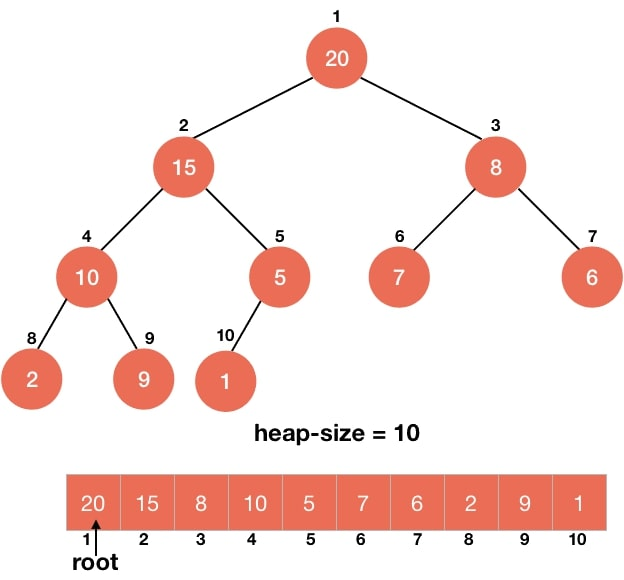
\includegraphics{heapsort.jpg}}
\end{center}
\end{frame}



\begin{frame}
\frametitle{Postup}

\begin{enumerate}
\setlength\itemsep{0.3em}
 \item Vytvořit z listu hromadu.
 \item Vyměnit první prvek listu s posledním a snížit velikost listu o 1.
 \item Prosít prvek na jeho odpovídající index prostřednictvím zatřesení.
 \item Opakovat od kroku (2), dokud v listu nezůstane 1 prvek
\end{enumerate}

\end{frame}



\begin{frame}
\frametitle{Pseudokód vytvoření haldy}

\begin{algorithmic}
\State $left \gets (MAX \textbf{div} 2)-1$
\State $right \gets MAX - 1$
\For{$ i \gets (left, 0)^{-1}$} 
    \State $SiftDown(A,i,right)$
    
\EndFor 
\end{algorithmic}

\end{frame}



\begin{frame}
\frametitle{Pseudokód těla Heap-sortu}

\begin{algorithmic}
\For{$ right \gets (MAX-1, 1)^{-1}$} 
    \State $A[0] \leftrightarrow A[right]$
    \State $SiftDown(A,0,right-1)$
\EndFor 

\end{algorithmic}

\end{frame}



\begin{frame}
\frametitle{Složitost}
\begin{itemize}
\setlength\itemsep{0.5em}
 \item Zatřesení pracuje na složitosti $O(log_2n)$
 \item Pokud tedy se všemi prvky zatřeseme a následně prvek odebreme, vznikne složitost $O(n \hspace{0.25em} log_2n)$
\end{itemize}
\end{frame}
% $O(n \hspace{0.25em} log_n)$
\end{document}